%\VignetteEngine{knitr::knitr}
%\VignetteIndexEntry{Flexible Logo plots of symbols and alphanumeric strings using Logolas}
%\VignettePackage{Logolas}

% To compile this document
% library('knitr'); rm(list=ls()); knit('Logolas/vignettes/logolas.Rnw')
% library('knitr'); rm(list=ls()); knit2pdf('Logolas/vignettes/logolas.Rnw'); openPDF('logolas.pdf')
% !Rnw weave = knitr

\documentclass[12pt]{article}\usepackage[]{graphicx}\usepackage[usenames,dvipsnames]{color}
%% maxwidth is the original width if it is less than linewidth
%% otherwise use linewidth (to make sure the graphics do not exceed the margin)
\makeatletter
\def\maxwidth{ %
  \ifdim\Gin@nat@width>\linewidth
    \linewidth
  \else
    \Gin@nat@width
  \fi
}
\makeatother

\definecolor{fgcolor}{rgb}{0.251, 0.251, 0.251}
\newcommand{\hlnum}[1]{\textcolor[rgb]{0.816,0.125,0.439}{#1}}%
\newcommand{\hlstr}[1]{\textcolor[rgb]{0.251,0.627,0.251}{#1}}%
\newcommand{\hlcom}[1]{\textcolor[rgb]{0.502,0.502,0.502}{\textit{#1}}}%
\newcommand{\hlopt}[1]{\textcolor[rgb]{0,0,0}{#1}}%
\newcommand{\hlstd}[1]{\textcolor[rgb]{0.251,0.251,0.251}{#1}}%
\newcommand{\hlkwa}[1]{\textcolor[rgb]{0.125,0.125,0.941}{#1}}%
\newcommand{\hlkwb}[1]{\textcolor[rgb]{0,0,0}{#1}}%
\newcommand{\hlkwc}[1]{\textcolor[rgb]{0.251,0.251,0.251}{#1}}%
\newcommand{\hlkwd}[1]{\textcolor[rgb]{0.878,0.439,0.125}{#1}}%
\let\hlipl\hlkwb

\newenvironment{knitrout}{}{} % an empty environment to be redefined in TeX
\usepackage{alltt}

\newcommand{\Logolas}{\textit{Logolas}}
\usepackage{dsfont}
\usepackage{cite}



\RequirePackage[]{/Library/Frameworks/R.framework/Versions/3.4/Resources/library/BiocStyle/resources/tex/Bioconductor2}
\AtBeginDocument{\bibliographystyle{/Library/Frameworks/R.framework/Versions/3.4/Resources/library/BiocStyle/resources/tex/unsrturl}}



\author{Kushal K Dey, Dongyue Xie, Matthew Stephens  \\[1em]
\small{Dept. of Statistics, The University of Chicago} \mbox{ }\\
\small{\texttt{$^*$Correspondending Email: kkdey@uchicago.edu}}}


\bioctitle[ Enrichment Depletion Logo plots with String symbols using \Logolas{}]{Enrichment Depletion Logo plots with String symbols using \Logolas{}}
\IfFileExists{upquote.sty}{\usepackage{upquote}}{}
\begin{document}

\maketitle

\begin{abstract}
\vspace{1em}
Sequence logo plots have become a standard graphical tool for visualizing sequence motifs in DNA, RNA or protein sequences. However standard logo plots primarily highlight enrichment of symbols, and may fail to highlight interesting depletions. Current alternatives that try to highlight depletion often produce visually cluttered logos. We introduce a new sequence logo plot, the EDLogo plot, that highlights both enrichment and depletion, while minimizing visual clutter. We provide an easy-to-use and highly customizable R package Logolas to produce a range of logo plots, including EDLogo plots. This software also allows elements in the logo plot to be strings of characters, rather than a single character, extending the range of applications beyond the usual DNA, RNA or protein sequences. We illustrate our methods and software on applications to transcription factor binding site motifs, protein sequence alignments and cancer mutation signature profiles. Our new EDLogo plots, and flexible software implementation, can help data analysts visualize both enrichment and depletion of characters (DNA sequence bases, amino acids, etc) across a wide range of applications.

\vspace{1em}
\textbf{\Logolas{} version:} 2.0.1 \footnote{This document used the vignette from \Bioconductor{} package \Biocpkg{CountClust, DESeq2} as \CRANpkg{knitr} template}
\end{abstract}



\newpage

\tableofcontents

\section{Introduction}


Compared to the existing packages for plotting sequence logos (\textit{seqLogo}, \textit{seq2Logo}, \textit{motifStack} etc), \Logolas{} offers several new features that makes  logo visualization a more generic tool with potential applications in a much wider scope of problems.

- \textbf{Enrichment Depletion Logo (EDLogo)} : General logo plotting softwares highlight only enrichment of certain symbols, but Logolas allows the user to highlight both enrichment and depletion of symbols at any position, leading to more parsimonious and visually appealing representation.

- \textbf{String symbols} : General logo building softwares have limited library of symbols usually restricted to English alphabets. Logolas allows the user to plot symbols for any alphanumeric string, comprising of English alphabets, numbers, punctuation marks, arrows etc. It also provides an easy interface for the user to create her own logo and add to the library of symbols that can be plotted.

- \textbf{Dirichlet Adaptive Shrinkage} : Logolas provides a statistical approach to adaptively scale the heights of the logos based on the number of aligned sequences.

- \textbf{Better customizations} : Logolas offers several new color palettes, fill and border styles, several options for determining heights of the logos etc. Also, they can be plotted in multiple panels and combined with ggplot2 graphics.


\newpage

\section{\Logolas{} Installation}

\Logolas{} loads as dependencies the following CRAN-R package : \CRANpkg{grid}, \CRANpkg{gridExtra}, \CRANpkg{SQUAREM},  \CRANpkg{LaplacesDemon}, \CRANpkg{Matrix}, \CRANpkg{RColorBrewer}.

The Bioc version of \Logolas{} can be installed as follows

\begin{knitrout}
\definecolor{shadecolor}{rgb}{0.941, 0.941, 0.941}\color{fgcolor}\begin{kframe}
\begin{alltt}
\hlkwd{source}\hlstd{(}\hlstr{"http://bioconductor.org/biocLite.R"}\hlstd{)}
\hlkwd{biocLite}\hlstd{(}\hlstr{"Logolas"}\hlstd{)}
\end{alltt}
\end{kframe}
\end{knitrout}

For installing the developmental version of \Logolas{} from Github, the user is required to have the \CRANpkg{devtools} package and then run the following command.

\begin{knitrout}
\definecolor{shadecolor}{rgb}{0.941, 0.941, 0.941}\color{fgcolor}\begin{kframe}
\begin{alltt}
\hlstd{devtools}\hlopt{::}\hlkwd{install_github}\hlstd{(}\hlstr{'kkdey/Logolas'}\hlstd{)}
\end{alltt}
\end{kframe}
\end{knitrout}

Load \Logolas{} into R

\begin{knitrout}
\definecolor{shadecolor}{rgb}{0.941, 0.941, 0.941}\color{fgcolor}\begin{kframe}
\begin{alltt}
\hlkwd{library}\hlstd{(Logolas)}
\end{alltt}
\end{kframe}
\end{knitrout}

\section{Data Type}

\subsection{Data Format}

\Logolas{} accepts two data formats as input

- a vector of aligned character sequences (may be DNA, RNA or amino acid sequences), each of same length (see Example 1 below)

- a positional frequency (weight) matrix, termed PFM (PWM), with the symbols to be plotted along the rows and the positions of aligned sequences, from which the matrix is generated, along the columns. (see Example 2)

\subsection{String Data example}

Consider aligned strings of characters

\begin{knitrout}
\definecolor{shadecolor}{rgb}{0.941, 0.941, 0.941}\color{fgcolor}\begin{kframe}
\begin{alltt}
\hlstd{sequence} \hlkwb{<-} \hlkwd{c}\hlstd{(}\hlstr{"CTATTGT"}\hlstd{,} \hlstr{"CTCTTAT"}\hlstd{,} \hlstr{"CTATTAA"}\hlstd{,} \hlstr{"CTATTTA"}\hlstd{,} \hlstr{"CTATTAT"}\hlstd{,} \hlstr{"CTTGAAT"}\hlstd{,}
              \hlstr{"CTTAGAT"}\hlstd{,} \hlstr{"CTATTAA"}\hlstd{,} \hlstr{"CTATTTA"}\hlstd{,} \hlstr{"CTATTAT"}\hlstd{,} \hlstr{"CTTTTAT"}\hlstd{,} \hlstr{"CTATAGT"}\hlstd{,}
              \hlstr{"CTATTTT"}\hlstd{,} \hlstr{"CTTATAT"}\hlstd{,} \hlstr{"CTATATT"}\hlstd{,} \hlstr{"CTCATTT"}\hlstd{,} \hlstr{"CTTATTT"}\hlstd{,} \hlstr{"CAATAGT"}\hlstd{,}
              \hlstr{"CATTTGA"}\hlstd{,} \hlstr{"CTCTTAT"}\hlstd{,} \hlstr{"CTATTAT"}\hlstd{,} \hlstr{"CTTTTAT"}\hlstd{,} \hlstr{"CTATAAT"}\hlstd{,} \hlstr{"CTTAGGT"}\hlstd{,}
              \hlstr{"CTATTGT"}\hlstd{,} \hlstr{"CTCATGT"}\hlstd{,} \hlstr{"CTATAGT"}\hlstd{,} \hlstr{"CTCGTTA"}\hlstd{,} \hlstr{"CTAGAAT"}\hlstd{,} \hlstr{"CAATGGT"}\hlstd{)}
\end{alltt}
\end{kframe}
\end{knitrout}

The logo plots (both standard and Enrichment Depletion Logo) can be plotted using the
\textbf{logomaker()} function.

\begin{figure}[h]
\begin{center}
\begin{knitrout}
\definecolor{shadecolor}{rgb}{0.941, 0.941, 0.941}\color{fgcolor}\begin{kframe}
\begin{alltt}
\hlkwd{logomaker}\hlstd{(sequence,} \hlkwc{type} \hlstd{=} \hlstr{"Logo"}\hlstd{)}
\end{alltt}
\end{kframe}\begin{adjustwidth}{\fltoffset}{0mm}

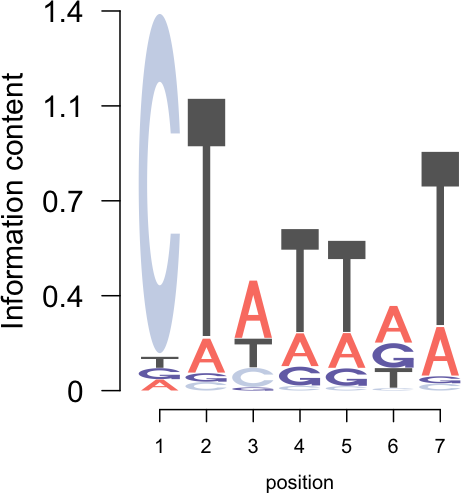
\includegraphics[width=4in,height=4in]{figure/standard_logo-1} \hfill{}

\end{adjustwidth}
\end{knitrout}
\end{center}
\end{figure}


\begin{figure}[h]
\begin{center}
\begin{knitrout}
\definecolor{shadecolor}{rgb}{0.941, 0.941, 0.941}\color{fgcolor}\begin{kframe}
\begin{alltt}
\hlkwd{logomaker}\hlstd{(sequence,} \hlkwc{type} \hlstd{=} \hlstr{"EDLogo"}\hlstd{)}
\end{alltt}
\end{kframe}\begin{adjustwidth}{\fltoffset}{0mm}

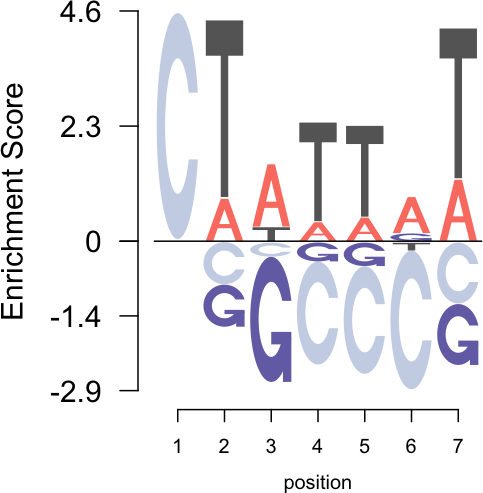
\includegraphics[width=4in,height=4in]{figure/ED_logo-1} \hfill{}

\end{adjustwidth}
\end{knitrout}
\end{center}
\end{figure}

\newpage

Instead of DNA.RNA sequqnce as above, one can also use amino acid character sequences.

\begin{figure}[h]
\begin{center}
\begin{knitrout}
\definecolor{shadecolor}{rgb}{0.941, 0.941, 0.941}\color{fgcolor}\begin{kframe}
\begin{alltt}
\hlkwd{library}\hlstd{(ggseqlogo)}
\hlkwd{data}\hlstd{(ggseqlogo_sample)}
\hlstd{sequence} \hlkwb{<-} \hlstd{seqs_aa}\hlopt{$}\hlstd{AKT1}
\hlkwd{logomaker}\hlstd{(sequence,} \hlkwc{type} \hlstd{=} \hlstr{"EDLogo"}\hlstd{)}
\end{alltt}
\end{kframe}\begin{adjustwidth}{\fltoffset}{0mm}

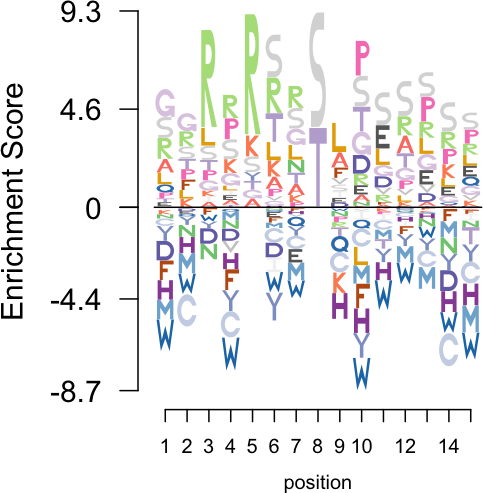
\includegraphics[width=4in,height=4in]{figure/ED_logo_2-1} \hfill{}

\end{adjustwidth}
\end{knitrout}
\end{center}
\end{figure}


\newpage
\subsection{Positional Frequency (Weight) Matrix}

We now see an example of positional weight matrix (PWM) as input to \textbf{logomaker()}.

\begin{knitrout}
\definecolor{shadecolor}{rgb}{0.941, 0.941, 0.941}\color{fgcolor}\begin{kframe}
\begin{alltt}
\hlkwd{data}\hlstd{(seqlogo_example)}
\end{alltt}
\end{kframe}
\end{knitrout}

We plot the logo plots for this PWM matrix.


\begin{figure}[h]
\begin{center}
\begin{knitrout}
\definecolor{shadecolor}{rgb}{0.941, 0.941, 0.941}\color{fgcolor}\begin{kframe}
\begin{alltt}
\hlkwd{logomaker}\hlstd{(seqlogo_example,} \hlkwc{type} \hlstd{=} \hlstr{"Logo"}\hlstd{,} \hlkwc{return_heights} \hlstd{=} \hlnum{TRUE}\hlstd{)}
\end{alltt}
\end{kframe}\begin{adjustwidth}{\fltoffset}{0mm}

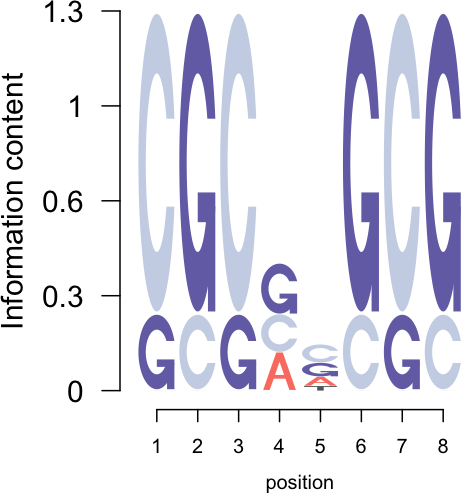
\includegraphics[width=4in,height=4in]{figure/logo_3-1} \hfill{}

\end{adjustwidth}\begin{kframe}\begin{verbatim}
## [1] 1.275 1.275 1.275 0.428 0.153 1.275 1.275 1.275
\end{verbatim}
\end{kframe}
\end{knitrout}
\end{center}
\end{figure}

\begin{figure}[h]
\begin{center}
\begin{knitrout}
\definecolor{shadecolor}{rgb}{0.941, 0.941, 0.941}\color{fgcolor}\begin{kframe}
\begin{alltt}
\hlkwd{logomaker}\hlstd{(seqlogo_example,} \hlkwc{type} \hlstd{=} \hlstr{"EDLogo"}\hlstd{,} \hlkwc{return_heights} \hlstd{=} \hlnum{TRUE}\hlstd{)}
\end{alltt}
\end{kframe}\begin{adjustwidth}{\fltoffset}{0mm}

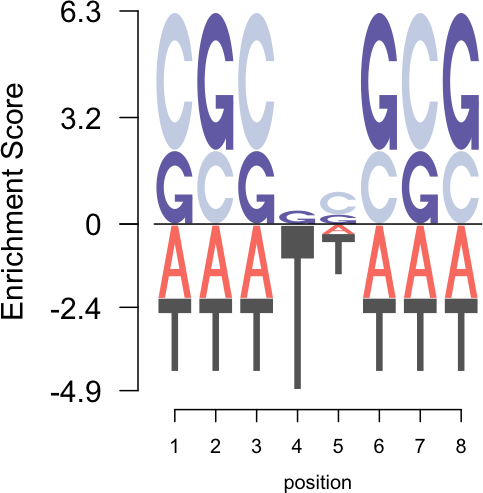
\includegraphics[width=4in,height=4in]{figure/edlogo_3-1} \hfill{}

\end{adjustwidth}\begin{kframe}\begin{verbatim}
## $pos_ic
##     1     2     3     4     5     6     7     8 
## 6.311 6.311 6.311 0.403 0.965 6.311 6.311 6.311 
## 
## $neg_ic
##    1    2    3    4    5    6    7    8 
## 4.36 4.36 4.36 4.93 1.49 4.36 4.36 4.36 
## 
## $table_mat_pos_norm
##       1     2     3 4     5     6     7     8
## A 0.000 0.000 0.000 0 0.000 0.000 0.000 0.000
## C 0.654 0.346 0.654 0 0.709 0.346 0.654 0.346
## G 0.346 0.654 0.346 1 0.291 0.654 0.346 0.654
## T 0.000 0.000 0.000 0 0.000 0.000 0.000 0.000
## 
## $table_mat_neg_norm
##     1   2   3 4     5   6   7   8
## A 0.5 0.5 0.5 0 0.188 0.5 0.5 0.5
## C 0.0 0.0 0.0 0 0.000 0.0 0.0 0.0
## G 0.0 0.0 0.0 0 0.000 0.0 0.0 0.0
## T 0.5 0.5 0.5 1 0.812 0.5 0.5 0.5
\end{verbatim}
\end{kframe}
\end{knitrout}
\end{center}
\end{figure}

The \begin{verb} return_heights = TRUE \end{verb} outputs the information content at each position for the standard logo plot (type = "Logo") and the heights of the stacks along the positive and negative Y axis, along
with the breakdown of the height due to different characters for the EDLogo plot (type = "EDLogo").

\clearpage

\section{Configuring Logos}

\subsection{Coloring schemes}

The \textbf{logomaker()} function provides three arguments to set the colors for the logos, a \begin{verb} color_type \end{verb} specifying the scheme of coloring used, \begin{verb} colors \end{verb} denoting the cohort of colors used and a \begin{verb} color_seed \end{verb} argument determining how sampling is done from this cohort.

The \begin{verb} color_type \end{verb} argument can be of three types, \begin{verb} per_row \end{verb}, \begin{verb} per_column \end{verb} and \begin{verb} per_symbol \end{verb}. \textbf{colors} element is a cohort of colors (chosen suitably large) from which distinct colors are chosen based on distinct \begin{verb} color_type \end{verb}. The number of colors chosen is of same length as number of rows in table for \begin{verb} per-row \end{verb} (assigning a color to each string), of same length as number of columns in table for \begin{verb} per-column \end{verb} (assuming a color for each column), or a distinct color for a distinct symbol in \begin{verb} per-symbol \end{verb}. The length of \textbf{colors} should be as large as the number of colors to be chosen in each scenario.
%
The default \begin{verb} color_type \end{verb} is \begin{verb} per-row \end{verb} and default \textbf{colors} comprises of a large cohort of nearly 70 distinct colors from which colors are sampled using the \begin{verb} color_seed \end{verb} argument.

\begin{knitrout}
\definecolor{shadecolor}{rgb}{0.941, 0.941, 0.941}\color{fgcolor}\begin{kframe}
\begin{alltt}
\hlkwd{logomaker}\hlstd{(seqlogo_example,} \hlkwc{color_type} \hlstd{=} \hlstr{"per_row"}\hlstd{,}
          \hlkwc{colors} \hlstd{=} \hlkwd{c}\hlstd{(}\hlstr{"#7FC97F"}\hlstd{,} \hlstr{"#BEAED4"}\hlstd{,} \hlstr{"#FDC086"}\hlstd{,} \hlstr{"#386CB0"}\hlstd{),}
          \hlkwc{type} \hlstd{=} \hlstr{"EDLogo"}\hlstd{)}
\end{alltt}
\end{kframe}\begin{adjustwidth}{\fltoffset}{0mm}

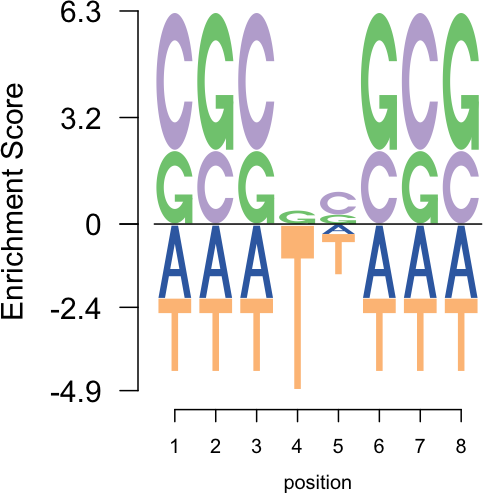
\includegraphics[width=4in,height=4in]{figure/col_prof-1} \hfill{}

\end{adjustwidth}\begin{kframe}\begin{alltt}
\hlkwd{logomaker}\hlstd{(seqlogo_example,} \hlkwc{type} \hlstd{=} \hlstr{"EDLogo"}\hlstd{,} \hlkwc{color_seed} \hlstd{=} \hlnum{1500}\hlstd{)}
\end{alltt}
\end{kframe}\begin{adjustwidth}{\fltoffset}{0mm}

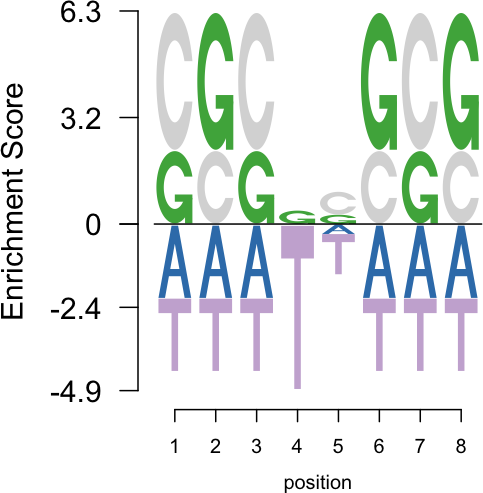
\includegraphics[width=4in,height=4in]{figure/col_prof-2} \hfill{}

\end{adjustwidth}
\end{knitrout}

\subsection{Styles of symbols}

Besides the default style with filled symbols for each character, one can also use characters with border styles. For the standard logo plot, this is accomplished by the \begin{verb} tofill \end{verb} control argument.

\begin{knitrout}
\definecolor{shadecolor}{rgb}{0.941, 0.941, 0.941}\color{fgcolor}\begin{kframe}
\begin{alltt}
\hlkwd{logomaker}\hlstd{(seqlogo_example,} \hlkwc{type} \hlstd{=} \hlstr{"Logo"}\hlstd{,}
          \hlkwc{logo_control} \hlstd{=} \hlkwd{list}\hlstd{(}\hlkwc{control} \hlstd{=} \hlkwd{list}\hlstd{(}\hlkwc{tofill}\hlstd{=} \hlnum{FALSE}\hlstd{)))}
\end{alltt}
\end{kframe}\begin{adjustwidth}{\fltoffset}{0mm}

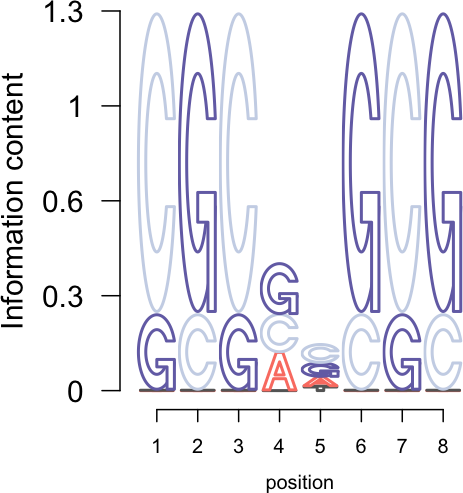
\includegraphics[width=4in,height=4in]{figure/fill-1} \hfill{}

\end{adjustwidth}
\end{knitrout}

For an EDLogo plot, the arguments \begin{verb} tofill_pos \end{verb} and \begin{verb} tofill_neg \end{verb} represent the coloring scheme for the positive and the negative axes in an EDLogo plot.

\begin{knitrout}
\definecolor{shadecolor}{rgb}{0.941, 0.941, 0.941}\color{fgcolor}\begin{kframe}
\begin{alltt}
\hlkwd{logomaker}\hlstd{(seqlogo_example,} \hlkwc{type} \hlstd{=} \hlstr{"EDLogo"}\hlstd{,}
          \hlkwc{logo_control} \hlstd{=} \hlkwd{list}\hlstd{(}\hlkwc{control} \hlstd{=} \hlkwd{list}\hlstd{(}\hlkwc{tofill_pos} \hlstd{=} \hlnum{TRUE}\hlstd{,}
                                             \hlkwc{tofill_neg} \hlstd{=} \hlnum{FALSE}\hlstd{)))}
\end{alltt}
\end{kframe}\begin{adjustwidth}{\fltoffset}{0mm}

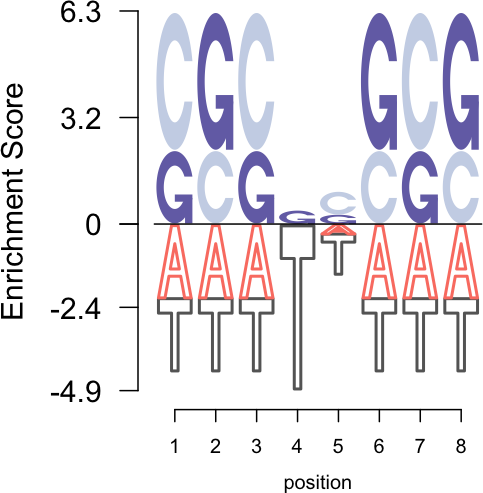
\includegraphics[width=4in,height=4in]{figure/fill2-1} \hfill{}

\end{adjustwidth}
\end{knitrout}


\subsection{Background Info}

\Logolas{} allows the user to scale the data based on a specified background information. The background information can be incorporated in the argument \begin{verb} bg \end{verb}. The default value is NULL,
in which case equal probability is assigned to each symbol. The user can however specify a
vector (equal to in length to the number of symbols) which specifies the background probability
for each symbol and assumes this background probability to be the same across the columns (sites),
or a matrix, whose each cell specifies the background probability of the symbols for each position.

First example with \begin{verb} bg \end{verb} as a vector.

\begin{knitrout}
\definecolor{shadecolor}{rgb}{0.941, 0.941, 0.941}\color{fgcolor}\begin{kframe}
\begin{alltt}
\hlstd{bg} \hlkwb{<-} \hlkwd{c}\hlstd{(}\hlnum{0.05}\hlstd{,} \hlnum{0.90}\hlstd{,} \hlnum{0.03}\hlstd{,} \hlnum{0.05}\hlstd{)}
\hlkwd{names}\hlstd{(bg)} \hlkwb{<-} \hlkwd{c}\hlstd{(}\hlstr{"A"}\hlstd{,} \hlstr{"C"}\hlstd{,} \hlstr{"G"}\hlstd{,} \hlstr{"T"}\hlstd{)}
\hlkwd{logomaker}\hlstd{(seqlogo_example,} \hlkwc{bg}\hlstd{=bg,} \hlkwc{type} \hlstd{=} \hlstr{"EDLogo"}\hlstd{)}
\end{alltt}
\end{kframe}\begin{adjustwidth}{\fltoffset}{0mm}

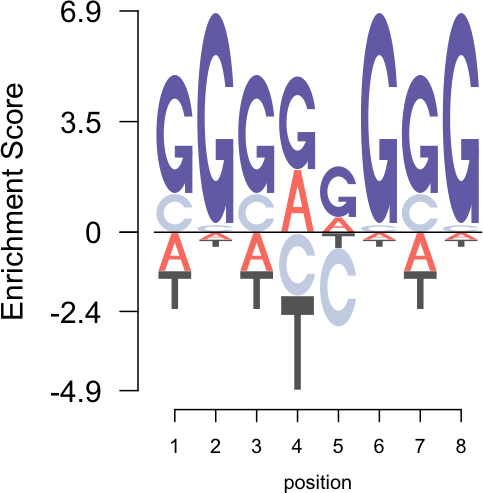
\includegraphics[width=4in,height=4in]{figure/bg-1} \hfill{}

\end{adjustwidth}
\end{knitrout}

Second example with \begin{verb} bg \end{verb} as a matrix.

\begin{knitrout}
\definecolor{shadecolor}{rgb}{0.941, 0.941, 0.941}\color{fgcolor}\begin{kframe}
\begin{alltt}
\hlkwd{logomaker}\hlstd{(seqlogo_example,} \hlkwc{bg}\hlstd{=(seqlogo_example}\hlopt{+}\hlnum{1e-02}\hlstd{),} \hlkwc{type} \hlstd{=} \hlstr{"EDLogo"}\hlstd{)}
\end{alltt}
\end{kframe}\begin{adjustwidth}{\fltoffset}{0mm}

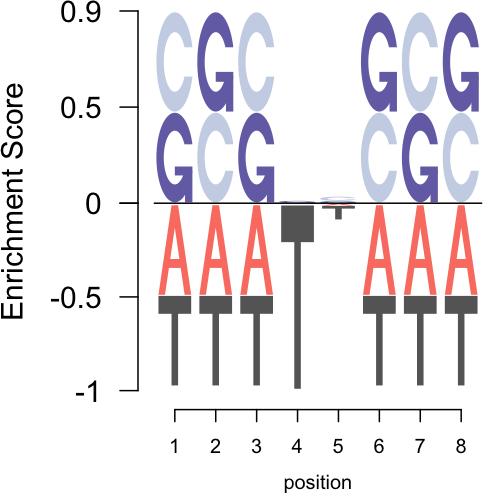
\includegraphics[width=4in,height=4in]{figure/bg2-1} \hfill{}

\end{adjustwidth}
\end{knitrout}

\section{Adaptive scaling of logos}

\Logolas{} allows the user to perform adaptive scaling of the stack heights in a logo plot based on the
number of aligned sequences, using the \begin{verb} use_dash \end{verb} argument. This scaling is performed
only when the data input into the \textbf{logomaker()} function is a vector of sequences or a position frequency (PFM) matrix. We show an example with and without the \begin{verb} use_dash \end{verb} argument.

\begin{knitrout}
\definecolor{shadecolor}{rgb}{0.941, 0.941, 0.941}\color{fgcolor}\begin{kframe}
\begin{alltt}
\hlstd{sequence} \hlkwb{<-} \hlkwd{c}\hlstd{(}\hlstr{"CTATTGT"}\hlstd{,} \hlstr{"CTCTTAT"}\hlstd{,} \hlstr{"CTATTAA"}\hlstd{,} \hlstr{"CTATTTA"}\hlstd{,} \hlstr{"CTATTAT"}\hlstd{,} \hlstr{"CTTGAAT"}\hlstd{,}
              \hlstr{"CTTAGAT"}\hlstd{,} \hlstr{"CTATTAA"}\hlstd{,} \hlstr{"CTATTTA"}\hlstd{,} \hlstr{"CTATTAT"}\hlstd{)}
\hlkwd{logomaker}\hlstd{(sequence,} \hlkwc{use_dash} \hlstd{=} \hlnum{FALSE}\hlstd{,} \hlkwc{type} \hlstd{=} \hlstr{"Logo"}\hlstd{,}
          \hlkwc{logo_control} \hlstd{=} \hlkwd{list}\hlstd{(}\hlkwc{pop_name} \hlstd{=} \hlstr{"use_dash = FALSE"}\hlstd{))}
\end{alltt}
\end{kframe}\begin{adjustwidth}{\fltoffset}{0mm}

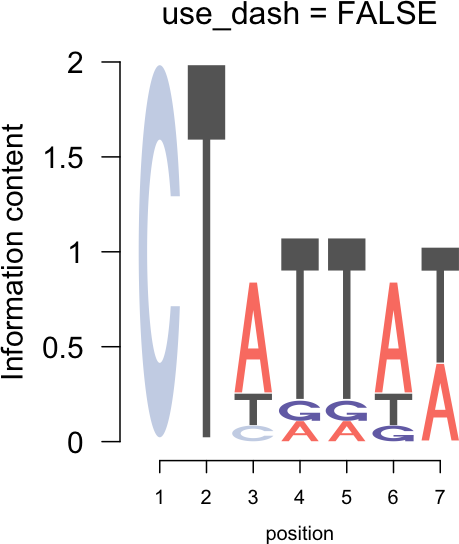
\includegraphics[width=4in,height=4in]{figure/dash-1} \hfill{}

\end{adjustwidth}\begin{kframe}\begin{alltt}
\hlkwd{logomaker}\hlstd{(sequence,} \hlkwc{type} \hlstd{=} \hlstr{"Logo"}\hlstd{,} \hlkwc{logo_control} \hlstd{=} \hlkwd{list}\hlstd{(}\hlkwc{pop_name} \hlstd{=} \hlstr{"use_dash = TRUE"}\hlstd{))}
\end{alltt}
\end{kframe}\begin{adjustwidth}{\fltoffset}{0mm}

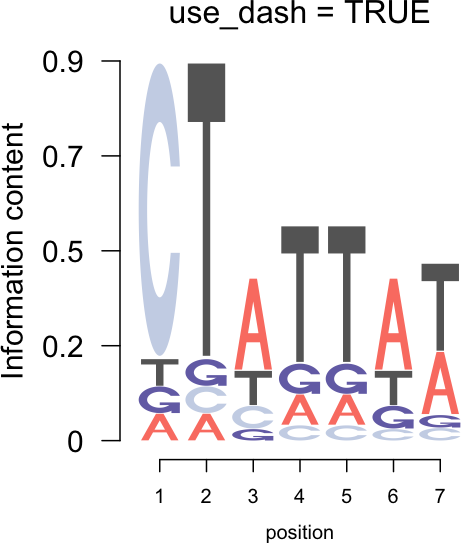
\includegraphics[width=4in,height=4in]{figure/dash-2} \hfill{}

\end{adjustwidth}
\end{knitrout}

The adaptive scaling is performed by the Dirichlet Adaptive Shrinkage method, the details of which can be viewed at our \textbf{dashr} package repository \url{https://github.com/kkdey/dashr}.

\section{String symbols}

\Logolas{} allows the user to plot symbols not just for characters as we saw in previous examples, but for any alphanumeric string. We present two examples - one for representing mutation signature and another for representing histone marks composition.

Histone marks string symbols example

\begin{knitrout}
\definecolor{shadecolor}{rgb}{0.941, 0.941, 0.941}\color{fgcolor}\begin{kframe}
\begin{alltt}
\hlkwd{data}\hlstd{(}\hlstr{"histone_marks"}\hlstd{)}
\hlkwd{logomaker}\hlstd{(histone_marks}\hlopt{$}\hlstd{mat,} \hlkwc{bg}\hlstd{=histone_marks}\hlopt{$}\hlstd{bgmat,} \hlkwc{type} \hlstd{=} \hlstr{"EDLogo"}\hlstd{)}
\end{alltt}
\end{kframe}\begin{adjustwidth}{\fltoffset}{0mm}

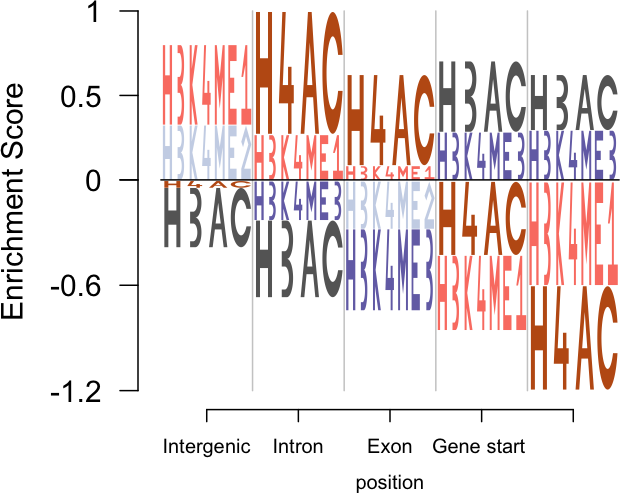
\includegraphics[width=5in,height=4in]{figure/histones-1} \hfill{}

\end{adjustwidth}
\end{knitrout}

Mutation signature string and character mix example.

\begin{knitrout}
\definecolor{shadecolor}{rgb}{0.941, 0.941, 0.941}\color{fgcolor}\begin{kframe}
\begin{alltt}
\hlkwd{data}\hlstd{(}\hlstr{"mutation_sig"}\hlstd{)}
\hlkwd{logomaker}\hlstd{(mutation_sig,} \hlkwc{type} \hlstd{=} \hlstr{"Logo"}\hlstd{,} \hlkwc{color_seed} \hlstd{=} \hlnum{3000}\hlstd{)}
\end{alltt}
\end{kframe}\begin{adjustwidth}{\fltoffset}{0mm}

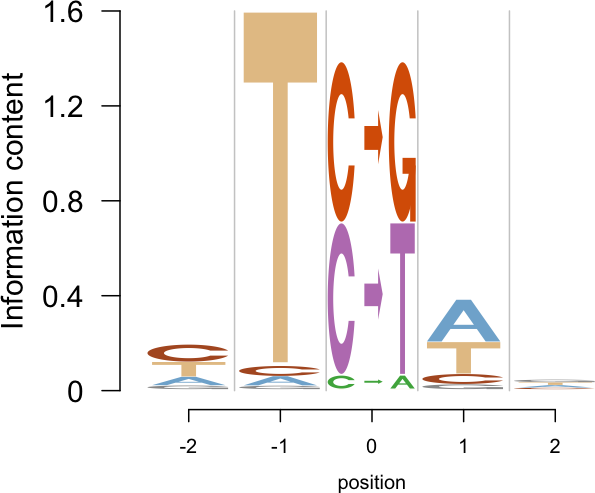
\includegraphics[width=5in,height=4in]{figure/mutsig2-1} \hfill{}

\end{adjustwidth}
\end{knitrout}

The user may want to have distinct colors for distinct symbols. This is where we use the \textit{persymbol}
option for  \begin{verb} color_type \end{verb}.

\begin{knitrout}
\definecolor{shadecolor}{rgb}{0.941, 0.941, 0.941}\color{fgcolor}\begin{kframe}
\begin{alltt}
\hlkwd{logomaker}\hlstd{(mutation_sig,} \hlkwc{type} \hlstd{=} \hlstr{"Logo"}\hlstd{,} \hlkwc{color_type} \hlstd{=} \hlstr{"per_symbol"}\hlstd{,}  \hlkwc{color_seed} \hlstd{=} \hlnum{2300}\hlstd{)}
\end{alltt}
\end{kframe}\begin{adjustwidth}{\fltoffset}{0mm}

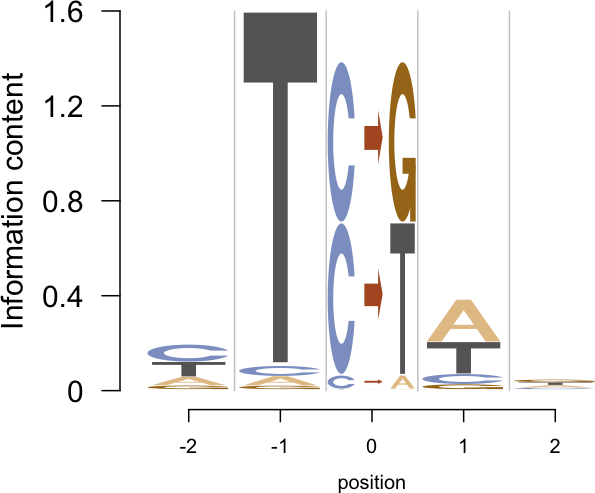
\includegraphics[width=5in,height=4in]{figure/mutsig3-1} \hfill{}

\end{adjustwidth}
\end{knitrout}

The corresponding EDLogo

\begin{knitrout}
\definecolor{shadecolor}{rgb}{0.941, 0.941, 0.941}\color{fgcolor}\begin{kframe}
\begin{alltt}
\hlkwd{logomaker}\hlstd{(mutation_sig,} \hlkwc{type} \hlstd{=} \hlstr{"EDLogo"}\hlstd{,} \hlkwc{color_type} \hlstd{=} \hlstr{"per_symbol"}\hlstd{,}  \hlkwc{color_seed} \hlstd{=} \hlnum{2300}\hlstd{)}
\end{alltt}
\end{kframe}\begin{adjustwidth}{\fltoffset}{0mm}

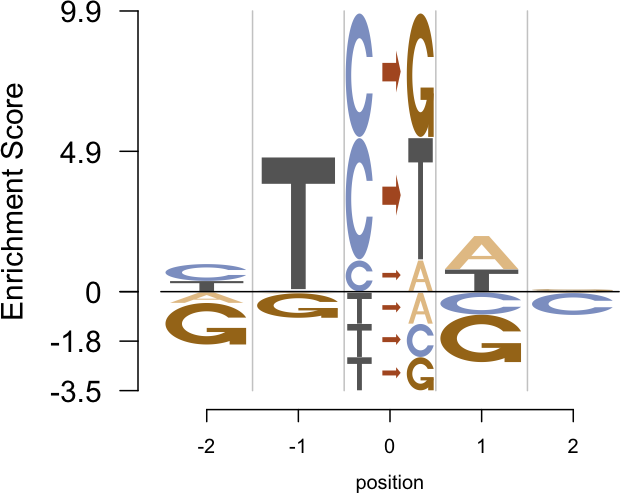
\includegraphics[width=5in,height=4in]{figure/mutsig4-1} \hfill{}

\end{adjustwidth}
\end{knitrout}


\section{Extras}

\subsection{Consensus Sequence}

\Logolas{} provides a new nomenclature to geneerate consensus sequence from a positional frequency (weight) matrix or from a vector of aligned sequences. This is performed by the \begin{verb} GetConsensusSeq() \end{verb} function.

\begin{knitrout}
\definecolor{shadecolor}{rgb}{0.941, 0.941, 0.941}\color{fgcolor}\begin{kframe}
\begin{alltt}
\hlstd{sequence} \hlkwb{<-} \hlkwd{c}\hlstd{(}\hlstr{"CTATTGT"}\hlstd{,} \hlstr{"CTCTTAT"}\hlstd{,} \hlstr{"CTATTAA"}\hlstd{,} \hlstr{"CTATTTA"}\hlstd{,} \hlstr{"CTATTAT"}\hlstd{,} \hlstr{"CTTGAAT"}\hlstd{,}
              \hlstr{"CTTAGAT"}\hlstd{,} \hlstr{"CTATTAA"}\hlstd{,} \hlstr{"CTATTTA"}\hlstd{,} \hlstr{"CTATTAT"}\hlstd{)}
\hlkwd{GetConsensusSeq}\hlstd{(sequence)}
\end{alltt}
\begin{verbatim}
## [1] "C T (Ag) T T (Ac) (TA)"
\end{verbatim}
\end{kframe}
\end{knitrout}

In the sequence, a position represented by (Ag) would mean enrichment in A and depletion in G at that position.
One can input a PWM or PFM matrix with A, C, G and T as row names in the \begin{verb} GetConsensusSeq() \end{verb} function as well.

\subsection{Multiple panels plots}

\Logolas{} plots can be plotted in multiple panels, as depicted below.

\begin{knitrout}
\definecolor{shadecolor}{rgb}{0.941, 0.941, 0.941}\color{fgcolor}\begin{kframe}
\begin{alltt}
\hlstd{sequence} \hlkwb{<-} \hlkwd{c}\hlstd{(}\hlstr{"CTATTGT"}\hlstd{,} \hlstr{"CTCTTAT"}\hlstd{,} \hlstr{"CTATTAA"}\hlstd{,} \hlstr{"CTATTTA"}\hlstd{,} \hlstr{"CTATTAT"}\hlstd{,} \hlstr{"CTTGAAT"}\hlstd{,}
              \hlstr{"CTTAGAT"}\hlstd{,} \hlstr{"CTATTAA"}\hlstd{,} \hlstr{"CTATTTA"}\hlstd{,} \hlstr{"CTATTAT"}\hlstd{)}
\hlstd{Logolas}\hlopt{::}\hlkwd{get_viewport_logo}\hlstd{(}\hlnum{1}\hlstd{,} \hlnum{2}\hlstd{,} \hlkwc{heights_1} \hlstd{=} \hlnum{20}\hlstd{)} \hlcom{## first arg: num of rows in panel, second arg: num of columns}
\hlkwd{library}\hlstd{(grid)}
\hlkwd{seekViewport}\hlstd{(}\hlkwd{paste0}\hlstd{(}\hlstr{"plotlogo"}\hlstd{,} \hlnum{1}\hlstd{))}
\hlkwd{logomaker}\hlstd{(sequence,} \hlkwc{type} \hlstd{=} \hlstr{"Logo"}\hlstd{,} \hlkwc{logo_control} \hlstd{=} \hlkwd{list}\hlstd{(}\hlkwc{newpage} \hlstd{=} \hlnum{FALSE}\hlstd{))}

\hlkwd{seekViewport}\hlstd{(}\hlkwd{paste0}\hlstd{(}\hlstr{"plotlogo"}\hlstd{,} \hlnum{2}\hlstd{))}
\hlkwd{logomaker}\hlstd{(sequence,} \hlkwc{type} \hlstd{=} \hlstr{"EDLogo"}\hlstd{,} \hlkwc{logo_control} \hlstd{=} \hlkwd{list}\hlstd{(}\hlkwc{newpage} \hlstd{=} \hlnum{FALSE}\hlstd{))}
\end{alltt}
\end{kframe}\begin{adjustwidth}{\fltoffset}{0mm}

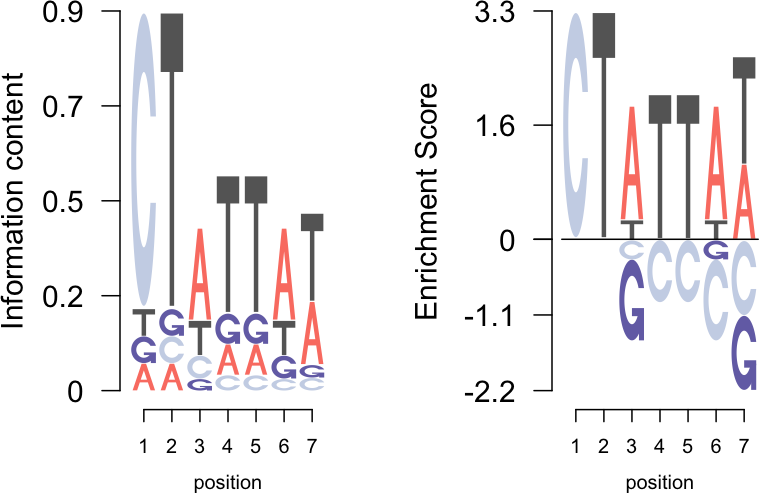
\includegraphics[width=6in,height=4in]{figure/mult_panels-1} \hfill{}

\end{adjustwidth}
\end{knitrout}

In the same way, ggplot2 graphics can also be combined with \Logolas{} plots.

\subsection {PSSM logos}

While \textbf{logomaker} takes a PFM, PWM or a set of aligned sequences as input, sometimes, some position specific scores are only available to the user. In this case, one can use the \begin{verb} logo_pssm() \end{verb}
in \Logolas{} to plot the scoring matrix.

\begin{knitrout}
\definecolor{shadecolor}{rgb}{0.941, 0.941, 0.941}\color{fgcolor}\begin{kframe}
\begin{alltt}
\hlkwd{data}\hlstd{(}\hlstr{"pssm"}\hlstd{)}
\hlkwd{logo_pssm}\hlstd{(pssm,} \hlkwc{control} \hlstd{=} \hlkwd{list}\hlstd{(}\hlkwc{round_off} \hlstd{=} \hlnum{0}\hlstd{))}
\end{alltt}
\end{kframe}\begin{adjustwidth}{\fltoffset}{0mm}

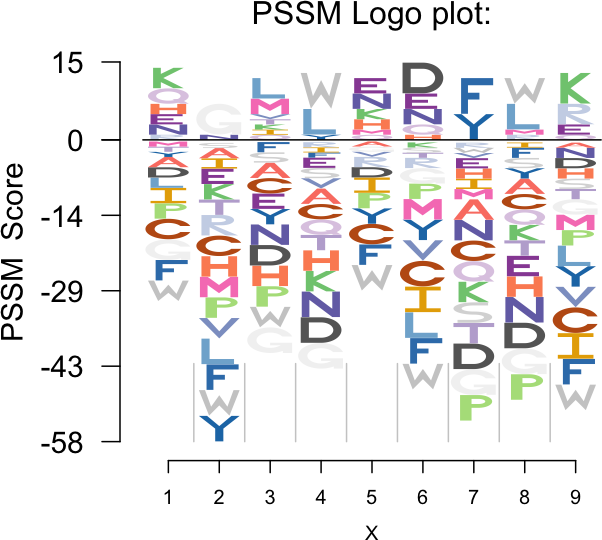
\includegraphics[width=5in,height=4in]{figure/pssm-1} \hfill{}

\end{adjustwidth}
\end{knitrout}

The \begin{verb} round_off \end{verb} comtrol argument specifies the number of points after decimal allowed in the axes of the plot.


\section{Acknowledgements}

The authors would like to acknowledge Oliver Bembom, the author of `seqLogo` for acting as an inspiration and providing the foundation on which this package is created. We also thank Peter Carbonetto, Edward Wallace and John Blischak for helpful feedback and discussions.

\section{Session Info}

\begin{knitrout}
\definecolor{shadecolor}{rgb}{0.941, 0.941, 0.941}\color{fgcolor}\begin{kframe}
\begin{alltt}
\hlkwd{sessionInfo}\hlstd{()}
\end{alltt}
\begin{verbatim}
## R version 3.4.2 (2017-09-28)
## Platform: x86_64-apple-darwin15.6.0 (64-bit)
## Running under: macOS Sierra 10.12.6
## 
## Matrix products: default
## BLAS: /Library/Frameworks/R.framework/Versions/3.4/Resources/lib/libRblas.0.dylib
## LAPACK: /Library/Frameworks/R.framework/Versions/3.4/Resources/lib/libRlapack.dylib
## 
## locale:
## [1] en_US.UTF-8/en_US.UTF-8/en_US.UTF-8/C/en_US.UTF-8/en_US.UTF-8
## 
## attached base packages:
## [1] grid      stats     graphics  grDevices utils     datasets  methods  
## [8] base     
## 
## other attached packages:
## [1] ggseqlogo_0.1 Logolas_2.0.1 knitr_1.17   
## 
## loaded via a namespace (and not attached):
##  [1] Rcpp_0.12.15         XVector_0.18.0       magrittr_1.5        
##  [4] zlibbioc_1.24.0      IRanges_2.12.0       BiocGenerics_0.24.0 
##  [7] munsell_0.4.3        gridBase_0.4-7       SQUAREM_2017.10-1   
## [10] colorspace_1.3-2     rlang_0.1.6          stringr_1.2.0       
## [13] highr_0.6            plyr_1.8.4           tools_3.4.2         
## [16] parallel_3.4.2       gtable_0.2.0         htmltools_0.3.6     
## [19] yaml_2.1.14          lazyeval_0.2.1       rprojroot_1.2       
## [22] digest_0.6.12        tibble_1.3.4         RColorBrewer_1.1-2  
## [25] ggplot2_2.2.1        S4Vectors_0.16.0     evaluate_0.10.1     
## [28] LaplacesDemon_16.1.0 rmarkdown_1.8        stringi_1.1.6       
## [31] compiler_3.4.2       Biostrings_2.46.0    scales_0.5.0        
## [34] backports_1.1.0      stats4_3.4.2         BiocStyle_2.6.0
\end{verbatim}
\end{kframe}
\end{knitrout}

\begin{thebibliography}{1}

\bibitem{Bembom2016}
Bembom O (2016).
\newblock seqLogo: Sequence logos for DNA sequence alignments.
\newblock R package version 1.40.0.

\bibitem{Wagih2014}
Omar Wagih (2014).
\newblock RWebLogo: plotting custom sequence logos.
\newblock R package version 1.0.3. https://CRAN.R-project.org/package=RWebLogo

\bibitem{Ou2015}
Jianhong Ou and Lihua Julie Zhu  (2015).
\newblock  motifStack: Plot stacked logos for single or multiple DNA, RNA and amino acid sequence.
\newblock  R package version 1.14.0.

\bibitem{Shiraishi2015}
Shiraishi Y, Tremmel G, Miyano S, Stephens M (2015)
\newblock A Simple Model-Based Approach to Inferring and Visualizing Cancer Mutation Signatures.
\newblock PLoS Genet 11(12): e1005657. doi: 10.1371/journal.pgen.1005657

\bibitem{Koch2007}
Koch CM, Andrews RM, Flicek P, et al (2007).
\newblock The landscape of histone modifications across $1 \%$ of the human genome in five human cell lines.
\newblock Genome Research. 2007;17(6):691-707. doi:10.1101/gr.5704207.

\end{thebibliography}

\end{document}
